\chapter{Unterkapitel}
\label{Abschnitt:Motivation}

\begin{figure}[H]
    \centering
    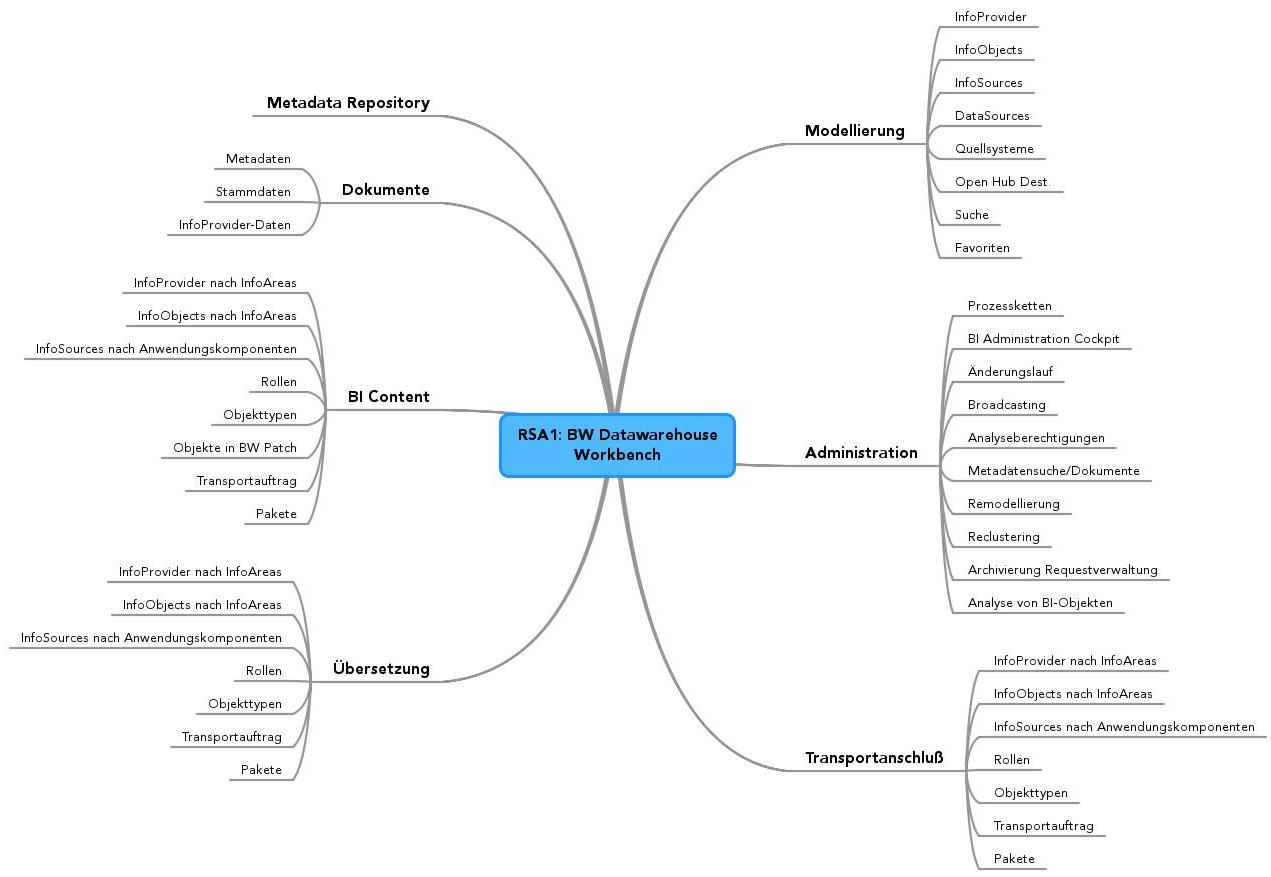
\includegraphics[width=1\textwidth]{files/RSA1Mindmap}
    \caption{Übersicht über RSA1}
    \label{pic:DWOverview}
\end{figure}


Die \textit{ Data Warehousing Workbench} lässt sich in die folgenden sieben Module unterteilen:\\


\begin{description}
\item[Modellierung:] Dieses Modul dient zur Modellierung von Daten und es werden verschiedene BI-Objekte bereitgestellt, welche zur Integration, Transformation, Konsolidierung, Bereinigung und Ablage von Daten genutzt werden können. Die verfügbaren BI-Objekte sind folgende:
\begin{itemize}
\item InfoProvider
Als InfoProvider werden verschiedene Metaobjekte der Datenbasis verstanden, die aus Sicht einer Querydefinition in uniformer Weise als Datenlieferanten betrachtet werden können und über deren Daten folglich auch in uniformer Weise berichtet werden kann. Die Art der Beschaffung der Daten, Detaillierungsgrad oder "Nähe" zum Quellsystem im Datenflussdiagramm ist dabei von InfoProvider zu InfoProvider verschieden. Im BEx Query Designer stehen sie allerdings als gleichwertige Objekte zur Verfügung. 

\item InfoCubes
Typ eines InfoProviders.
Ein InfoCube beschreibt einen (aus Sicht der Analyse) in sich geschlossenen Datenbestand z.B. eines betriebswirtschaftlichen Bereichs. Dieser Datenbestand kann mit der BEx Query ausgewertet werden. 
Ein InfoCube ist eine Menge von relationalen Tabellen, die nach dem Sternschema zusammengestellt sind: eine große Faktentabelle im Zentrum und mehrere sie umgebende Dimensionstabellen.
Verwendung
InfoCubes werden aus einer oder mehreren InfoSources oder aus anderen InfoProvidern mit Daten versorgt. Sie stehen dann als InfoProvider für die Analyse und Reporting zur Verfügung.


\item InfoSources
Grundsätzlich werden zwei Arten von InfoSources 3.x unterschieden:
-InfoSources mit flexibler Fortschreibung
-InfoSources mit direkter Fortschreibung
Bei beiden Typen werden die hochgeladenen Daten durch die Übertragungsregeln transformiert, die für die jeweilige Kombination von InfoSource und Quellsystem und für jedes InfoObject der Kommunikationsstruktur angelegt wurden. Ein InfoProvider kann von mehreren InfoSources versorgt werden, die wiederum von mehreren Quellsystemen versorgt werden können.


Bei einer InfoSource mit flexibler Fortschreibung werden die Daten aus der Kommunikationsstruktur unter Verwendung von Fortschreibungsregeln in die Datenziele (InfoCube, DataStore-Objekt, Stammdaten) geladen. Mehrere Datenziele können von einer InfoSource versorgt werden. Die InfoSource kann dabei Bewegungsdaten wie auch Stammdaten enthalten.

Mit einer InfoSource mit direkter Fortschreibung können Stammdaten (Merkmale mit Attributen, Texten oder Hierarchien) eines InfoObjects direkt (ohne Fortschreibungsregeln, nur unter Verwendung der Transferregeln) in die Stammdatentabelle fortgeschrieben werden. Dazu müssen Sie ihm eine Anwendungskomponente zuordnen. Das Merkmal erscheint daraufhin im InfoSource-Baum der Data Warehousing Workbench. Dort können Sie dem Merkmal DataSources und Quellsysteme zuordnen. Anschließend können Sie für das Merkmal Stammdaten, Texte und Hierarchien laden.

\end{itemize}
Die Grafische Oberfläche ist in Abb. x zu sehen.
\begin{figure}[H]
    \centering
    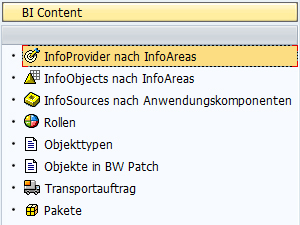
\includegraphics[width=0.5\textwidth]{files/BIContent}
    \caption{Das Modellierungsmenü}
    \label{pic:DWOverview}
\end{figure}
\item[Administration:] Hier befindet sich eine Ansicht für die verschiedensten Prozessketten, sowie das BI Administration Cockpit. Jenes wird verwendet, um die Performance von BI-Systemen zu überwachen. Es liefert einen zentralen Einstiegspunkt, sowie ein real-Time Monitoring und verschiedene Laufzeitstatistiken. Es bietet Zugriff auf Berichte und Anwendungen, die den Anwender bei der Ermittlung und Analyse von Problemen unterstützt. Es können BI-Objekte nachverfolgt und die Performance von BI-Aktivitäten optimiert werden.
Die Grafische Oberfläche ist in Abb. x zu sehen.
\begin{figure}[H]
    \centering
    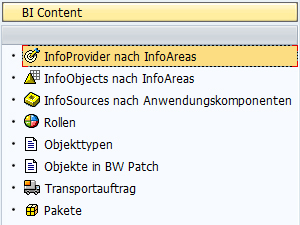
\includegraphics[width=0.5\textwidth]{files/BIContent}
    \caption{Das Administrationsmenü}
    \label{pic:DWOverview}
\end{figure}
\item[BI Content:] Die Struktur der verarbeiteten Geschäftsinformationen eines Unternehmens kann zu Auswertungszwecken im BI Content modelliert werden. Diese Modelle setzen sich aus verschiedenen Metadaten-Objekttypen zusammen. Hierbei werden vorkonfigurierte zur Analyse betriebswirtschaftlicher Fragestellungen verwendet. Wichtig hierbei ist, dass die Erzeugung, Verwendung, Überarbeitung und der Transport der BI-Objekte konsistent gehalten wird. Ein enthaltenes Konzept ist das \textit{BI-Versionskonzept} und eine Hauptfunktionalität ist die Übernahme von neuem BI Content in das Produktivsystem.
Die Grafische Oberfläche ist in Abb. xy zu sehen.
\begin{figure}[H]
    \centering
    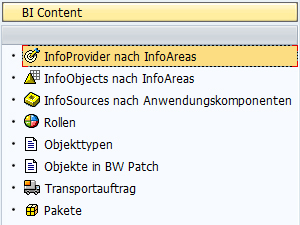
\includegraphics[width=0.5\textwidth]{files/BIContent}
    \caption{das BI Content Menü}
    \label{pic:DWOverview}
\end{figure}
\item[Transportanschluss:] Hier werden die selben Funktionalitäten wie in dem Modul \textit{BI Content} unterstützt, es besteht allerdings noch zusätzlich die Möglichkeit, BI-Objekte im XML-Format zu importieren bzw. zu exportieren.
Die Grafische Oberfläche ist in \textbf{Abb. \ref{pic:transport}} zu sehen.
\begin{figure}[H]
    \centering
    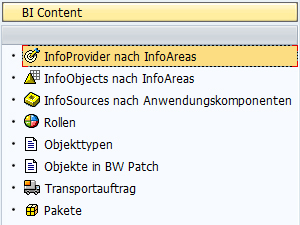
\includegraphics[width=0.5\textwidth]{files/BIContent}
    \caption{Transportanschluss}
    \label{pic:transport}
\end{figure}
\item[Dokumente:] Zu jedem BI-Objekt können jeweils ein oder mehrere Dokumente in verschiedenen Formaten, Versionen und Sprachen hinzugefügt, verlinkt und durchsucht werden. Diese Dokumente sind in drei Klassen unterteilt und können jeweils \textit{Metadaten}, \textit{Stammdaten} oder \textit{InfoProvider-Daten} zugeordnet werden.
Die Grafische Oberfläche ist in Abb. x zu sehen.
\begin{figure}[H]
    \centering
    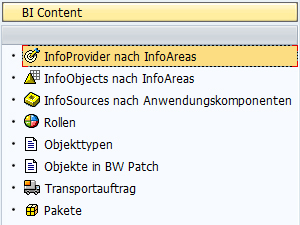
\includegraphics[width=0.5\textwidth]{files/BIContent}
    \caption{Das Dokumente Menü}
    \label{pic:DWOverview}
\end{figure}
\item[Übersetzung:] Um eine Internationalisierung umsetzen zu können, können mit Hilfe des Moduls \textit{Übersetzung} die Kurz- und Langtexte von BI-Metadaten-Objekten vereinfacht übersetzt werden. Zusätzlich kann die Übersetzungsumgebung, die der SAP Web Application Server (ABAP) beinhalted, verwendet werden.
Die Grafische Oberfläche ist in Abb. x zu sehen.
\begin{figure}[H]
    \centering
    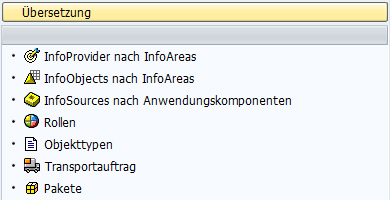
\includegraphics[width=0.5\textwidth]{files/Uebersetzung}
    \caption{Das Übersetzungsmenü}
    \label{pic:DWOverview}
\end{figure}
\item[Metadata Repository:] Das Metadata Repository basiert auf HTML und ermöglicht einen zentralen Zugriff auf Informationen von Metadaten-Objekten. Zu diesen Metadaten gehören zum Beispiel wichtige Eigenschaften der Objekte und die Verknüpfungen mit anderen Objekten.
\end{description}




